\section{Introduction}
\label{sec:noah__introduction}

The characterisation of small molecules and biomolecules by NMR spectroscopy relies on a suite of standard 2D NMR experiments, which seek to detect heteronuclear scalar couplings (e.g.\ HSQC and HMBC), homonuclear scalar couplings (e.g.\ COSY and TOCSY), or through-space interactions (e.g.\ NOESY and ROESY).
Although such 2D experiments provide far superior resolution and information content compared to 1D spectra, they also require substantially longer experimental durations, as the indirect dimension must be constructed through the acquisition of many $t_1$ increments.
This problem is further exacerbated by the fact that structural elucidation or verification often requires combined information from multiple different 2D experiments.

The acceleration of 2D NMR has thus proven to be a popular area of research.
We may broadly categorise these existing techniques into two classes.%
\footnote{These are by no means mutually exclusive: many of the techniques here can be combined to provide even greater efficiency.}
First come the methods which seek to directly speed up the acquisition of \textit{individual} 2D spectra: these include
\acf{nus}\autocite{Barna1987JMR,Kazimierczuk2010PNMRS,Mobli2014PNMRS,Kazimierczuk2015MRC},
fast pulsing (i.e.\ shortening of recovery delays)\autocite{SchulzeSunninghausen2014JACS,Schanda2006JACS,Kupce2007MRC,Schanda2009PNMRS},
ultrafast NMR\autocite{Frydman2002PNASUSA,Pelupessy2003JACS,Frydman2003JACS,Tal2010PNMRS,Gouilleux2018ARNMRS,Kupce2021NRMP},
Hadamard encoding\autocite{Kupce2003JMR,Kupce2003PNMRS},
and spectral aliasing\autocite{Jeannerat2000MRC,Bermel2009JACS,Njock2010C,Jeannerat2011eMR}.

On the other hand, \textit{multiple-FID experiments} aim to collect two or more 2D spectra in the time required for one.
The corresponding FIDs may either be detected at the same time (as in
time-shared NMR\autocite{Nolis2007ACIE,Parella2010CMR,Nolis2019JMR_psHSQC} and
multiple-receiver NMR\autocite{Kupce2006JACS,Kupce2008JACS,Kovacs2016MRC}),
or \textit{sequentially}: this is the category which NOAH supersequences\autocite{Kupce2017ACIE,Kupce2021PNMRS,Kupce2021NRMP} fall under.
NOAH supersequences are furthermore set apart from other sequential-acquisition experiments\autocite{Haasnoot1984JMR,Gurevich1984JMR,MotiramCorral2018CC,Nolis2019MRC,Nolis2019CPC,Nolis2019JMR} by their `modular' nature: they can be constructed from building blocks, or `modules', which (usually) contain one FID each.
Typically, each of these building blocks corresponds to a specific 2D experiment, as will be shown below.
It should be noted that there are several other multiple-FID experiments which, while not explicitly advertised as `NOAH experiments', are built from `modules' and are conceptually identical\autocite{Nagy2019CC,Nagy2020JMR,Nagy2021ACIE,Timari2022CC}; I do not discuss these here.

The time savings provided by NOAH experiments stems from the elision of \textit{recovery delays}---the time required for spins to relax to their equilibrium state ($\rho_0$ in \cref{eq:thermal_density_operator}), such that the next transient or $t_1$ increment can be recorded.
These recovery delays are responsible for most of the experimental duration of a typical 2D NMR experiment.
In a NOAH supersequence, this is accomplished by designing each module to draw on a different \textit{magnetisation pool}: this refers to a source of magnetisation belonging to a specific isotopologue.
For example, \carbon{}--bound protons and \carbont{}--bound protons are two different magnetisation pools.
This allows modules to be directly concatenated, without the addition of extra recovery delays between them; only one overall recovery delay is required for the entire supersequence, where \textit{all} magnetisation pools simultaneously recover.

In this section, I first provide a formal overview of how the time savings for NOAH experiments may be quantified and analysed.
This includes an analysis of the conditions under which multiple-FID techniques such as NOAH are most valuable.
Following this, I turn to the design of NOAH pulse sequences, using specific case studies to illustrate the general principles underlying these experiments.

\subsection{Time savings and sensitivity analyses}
\label{subsec:noah__snr}

\begin{figure}[htb]
    \centering
    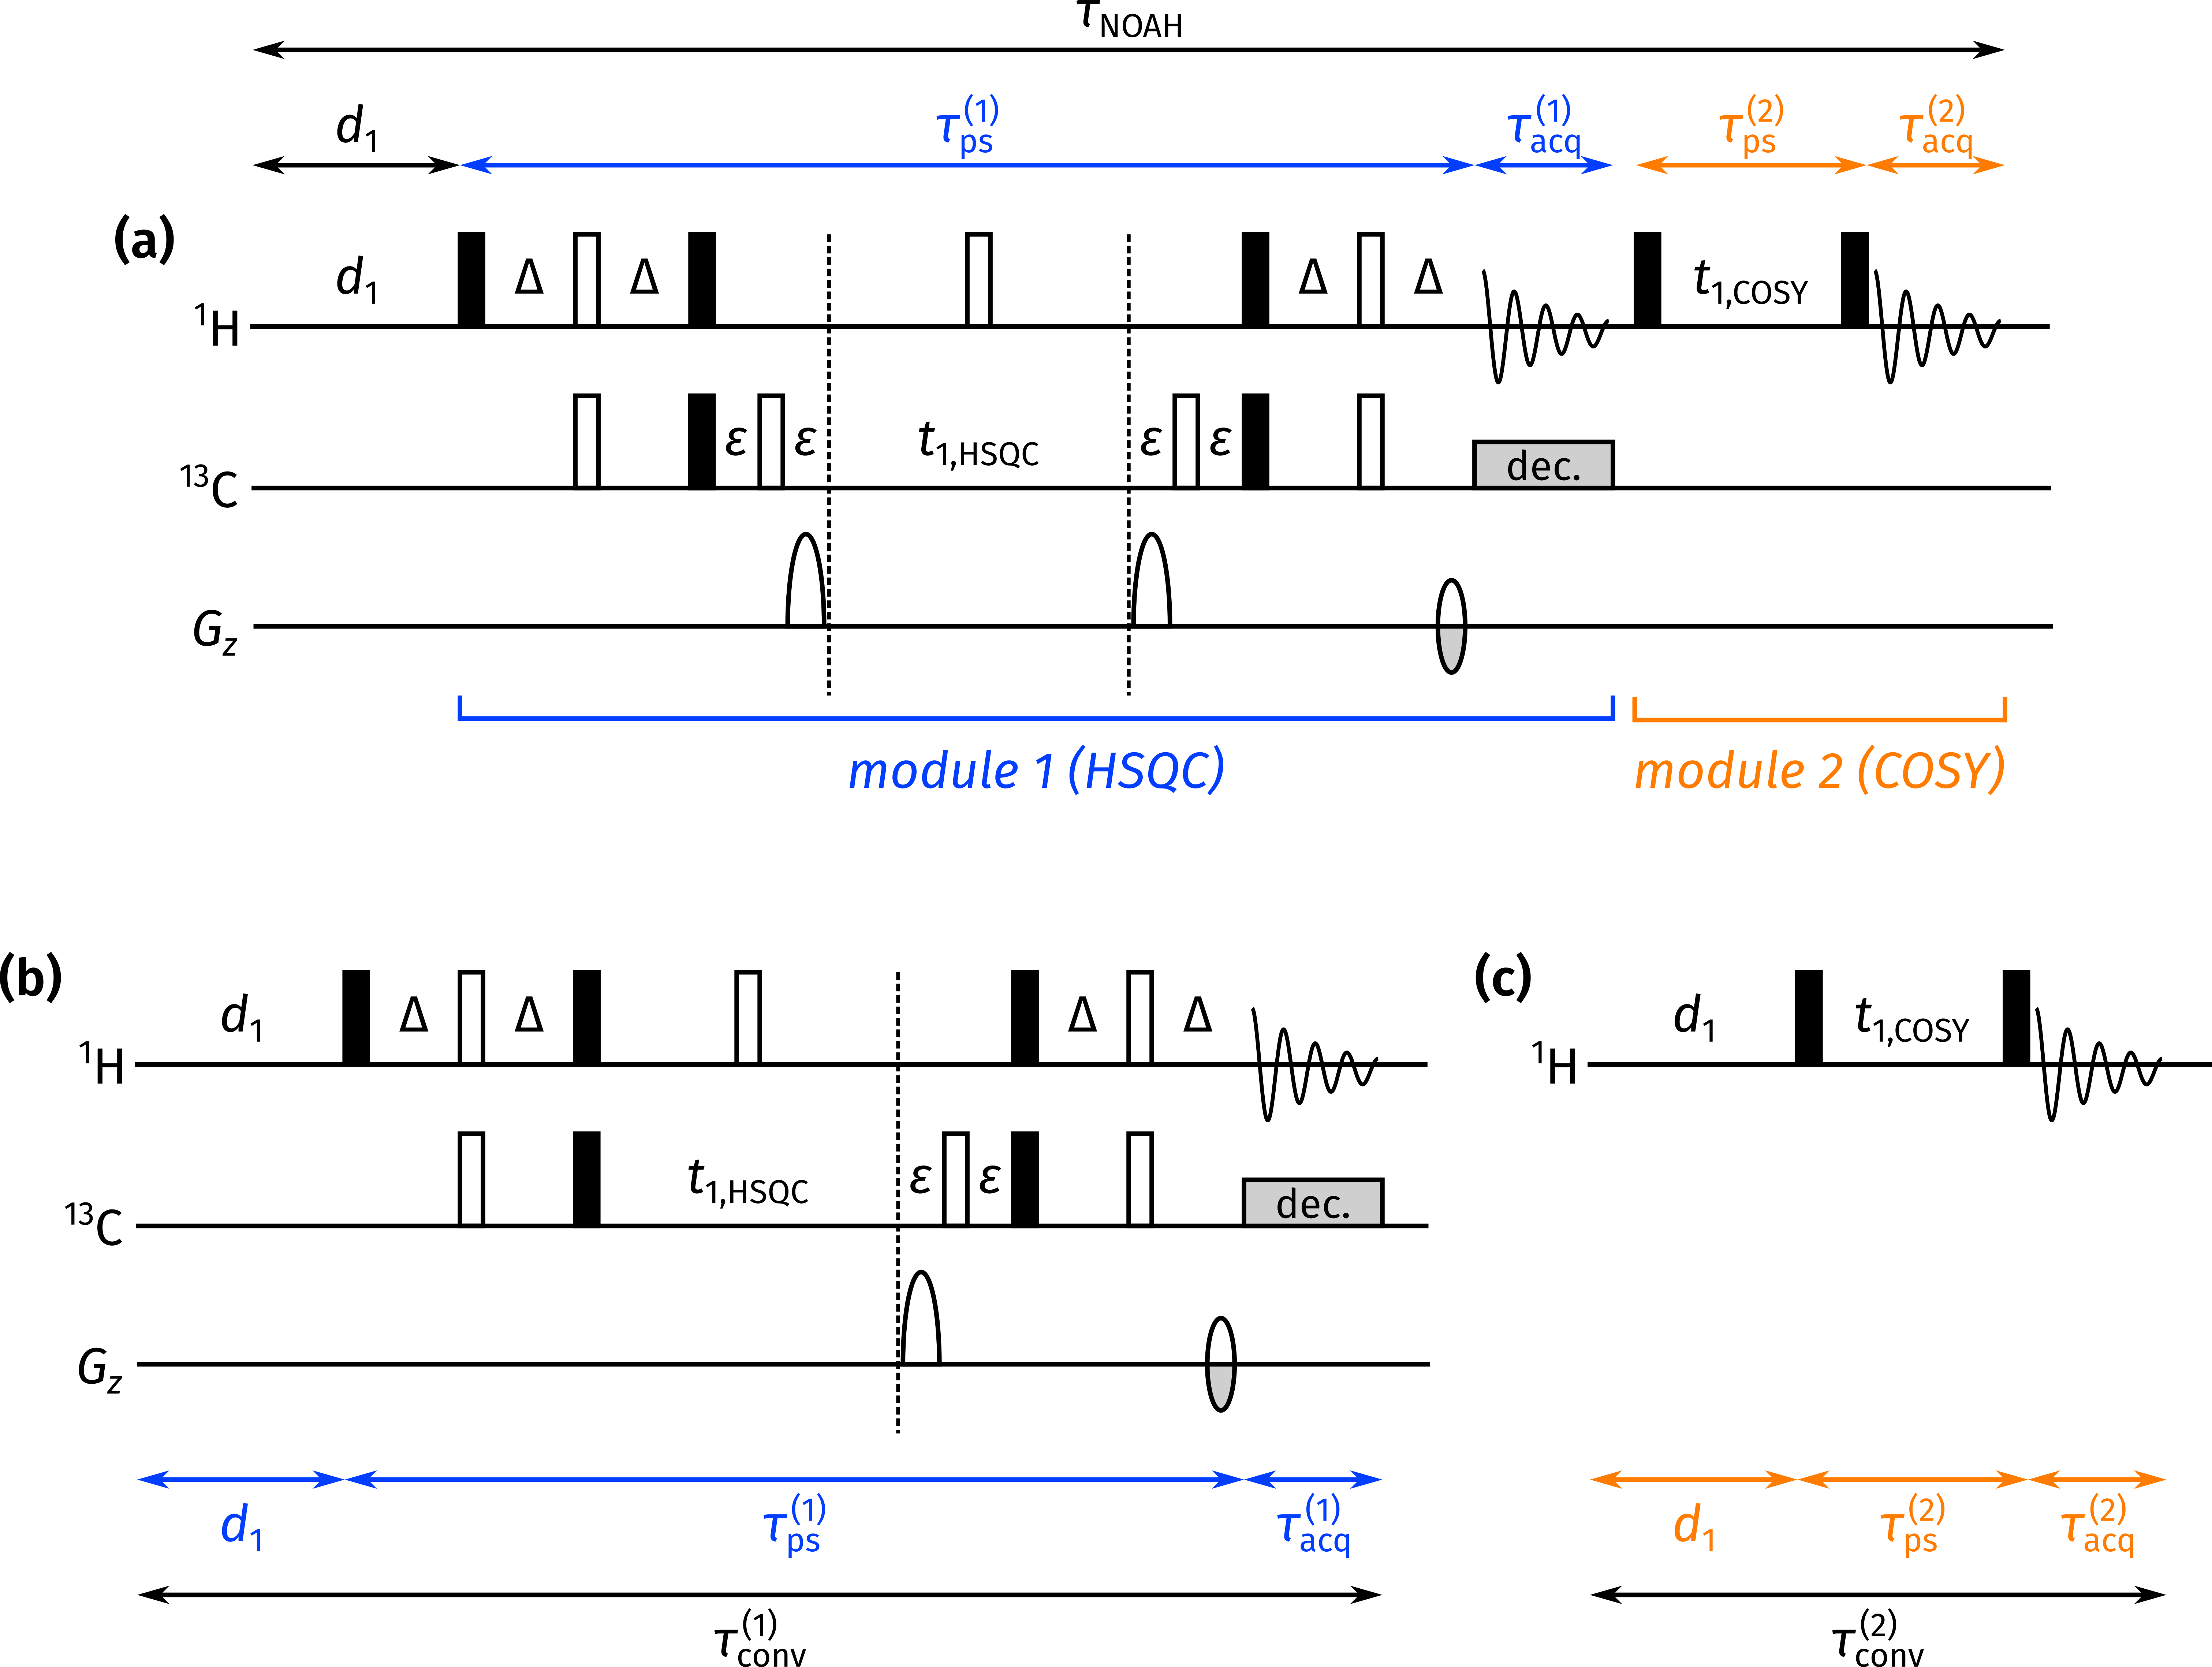
\includegraphics[]{noah/timings.png}%
    {\phantomsubcaption\label{fig:noah_timings_noah_sc}}%
    {\phantomsubcaption\label{fig:noah_timings_conv_s}}%
    {\phantomsubcaption\label{fig:noah_timings_conv_c}}%
    \caption[Comparison of NOAH and conventional 2D experiments]{
        \textbf{(\subref*{fig:noah_timings_noah_sc})} \noah{S,C} supersequence, comprising HSQC and COSY modules (see \cref{tbl:noah_modules} for an explanation of the single-letter module codes used).
        \textbf{(\subref*{fig:noah_timings_conv_s})} `Conventional' echo--antiecho HSQC (the same as in \cref{fig:hsqc_etgp}).
        \textbf{(\subref*{fig:noah_timings_conv_c})} `Conventional' COSY.
        The timings referred to in the text are highlighted for all three experiments; I have assumed that $d_1$ for each experiment is the same.
        Note that the lengths are not to scale: $d_1$ is typically far longer than the $\tau_\text{ps}$ and $\tau_\text{acq}$.
    }
    \label{fig:noah_timings}
\end{figure}

In a typical 2D NMR experiment, the majority of the experiment duration is taken up by the \textit{recovery delay}---the time required for spins to return to their equilibrium polarisation, such that the next transient or $t_1$ increment can be recorded.
The removal (or shortening) of recovery delays is thus a very effective way of speeding up 2D data acquisition.
In NOAH supersequences, 2D experiments (`modules') can be directly concatenated without the addition of extra recovery delays between them: only one overall recovery delay is required for the entire supersequence.
This means that, to a first approximation, a supersequence containing $N$ modules ($N \geq 2$) can be acquired in the time needed for just one module.
\Cref{fig:noah_timings} shows an example of a NOAH supersequence formed from two modules (HSQC and COSY): the various timings referred to in the text which follows are also marked on the diagram.

The duration of an NMR experiment, $\tau_\text{exp}$, can be expressed as a sum of its parts:
\begin{equation}
    \label{eq:exp_duration_2d}
    \tau_\text{exp} = \tau_\text{ps} + \tau_\text{acq} + d_1,
\end{equation}
where $\tau_\text{ps}$ is the time required for the pulse sequence itself (typically several milliseconds), $\tau_\text{acq}$ is the acquisition time (several hundred milliseconds), and $d_1$ is the recovery delay (one or more seconds).
The \textit{time-saving factor} $\rho_t$ for a NOAH supersequence, as compared to a series of conventional standalone experiments, is then:
\begin{equation}
    \label{eq:rho_t}
    \rho_t
    = \frac{\sum_i \tau_\text{conv}^{(i)}}{\tau_\text{NOAH}}
    = \frac{{\sum_i (\tau_\text{ps}^{(i)} + \tau_\text{acq}^{(i)} + d_1^{(i)})}}{d_1 + \sum_i (\tau_\text{ps}^{(i)} + \tau_\text{acq}^{(i)})},
\end{equation}
where $\tau_\text{NOAH}$ is the duration of the NOAH experiment, $\tau_\text{conv}$ is the duration of a conventional experiment, and the superscript $(i)$ represents the $i$-th module or conventional experiment being acquired.
The sum runs from $i = 1$ to $N$, where $N$ is the number of modules.
If we assume that $d_1^{(i)} = d_1$ is the same for all $N$ conventional experiments and the supersequence, then in the limit where
\begin{equation}
    \label{eq:d1_limit}
    d_1 \gg \sum_i \tau_\text{ps}^{(i)} + \tau_\text{acq}^{(i)},
\end{equation}
we have that $\rho_t \to Nd_1/d_1 = N$.
This analysis makes plenty of assumptions, and is not entirely valid in practice.
For example, \textit{each} $\tau_\text{acq}$ is often around 5\text{--}10\% of $d_1$, so is not entirely negligible, especially in longer supersequences.
Furthermore, some modules require longer $\tau_\text{ps}$: most notable is the NOESY module, which contains a mixing time of several hundred milliseconds. (HMBC, TOCSY, and ROESY spectra are also lesser offenders.)
These factors serve to reduce $\rho_t$ from its idealised value of $N$; generally, this deviation is larger as $N$ increases, because \cref{eq:d1_limit} becomes less and less valid.
Nevertheless, the general point that time savings are approximately proportional to $N$ stands.

For relatively concentrated samples, where sensitivity is not an issue, we can in fact end the discussion here.
In this \textit{sampling-limited regime}, the minimum 2D experiment duration is dictated purely by the number of $t_1$ increments needed to obtain sufficient resolution in the indirect dimension, as well as the minimum phase cycle required for artefact suppression.%
\footnote{With modern gradient-enhanced experiments, the minimum phase cycle may well not even be a `cycle'; see also \cref{fig:hsqc_comparison}.}
NOAH supersequences are identical to conventional experiments in both aspects, but provide a time-saving factor of $\rho_t \sim N$.

The development of modern NMR instrumentation, including high-field magnets and cryogenic probes, means that the sampling-limited regime continues to be extended to ever lower concentrations.
However, it is often not this simple: the opposite \textit{sensitivity-limited regime} is still very commonly encountered, for example with naturally insensitive experiments (e.g.\ ADEQUATE), low-field benchtop NMR, or most simply, dilute samples.%
\footnote{If the SNR factor $A^{(i)}$ as discussed below is \textit{very small}, then it is possible that even concentrated samples may be shifted into the sensitivity-limited regime. This is never really the case in practice, though, as will be shown in \cref{subsec:noah__case_studies}.}

In such cases, it becomes mandatory to compare the SNRs of the NOAH modules and conventional experiments.
To do so, we define for each module an \textit{SNR factor} $A^{(i)}$, which is the SNR of the NOAH module divided by the SNR of a conventional experiment, acquired with the same parameters.%
\footnote{The relative SNR will likely vary from peak to peak in the spectrum, and $A^{(i)}$ should in theory be quoted either as an average over all peaks, or as a range. This is what I have done in this thesis. However, comparisons in the literature are not always as thorough.}
In general, we have that $A \leq 1$, because NOAH modules frequently contain small modifications from conventional experiments (as will be explained in \cref{subsec:noah__magpools}).
The \textit{gain in sensitivity per unit time}, $\varepsilon^{(i)}$, is then defined by
\begin{equation}
    \label{eq:varepsilon_i}
    \varepsilon^{(i)} = A^{(i)} \sqrt{\rho_t},
\end{equation}
where the square root accounts for the fact that SNR scales only as the square root of the number of scans, or the number of times the experiment can be repeated in a given period.
Of course, the exact values calculated for $A^{(i)}$ (and hence $\varepsilon^{(i)}$) will depend on the sample chosen for the comparison.
These values should therefore be assumed to be valid only for similar samples.

If $\varepsilon^{(i)} > 1$, as is frequently the case, this means that the NOAH supersequence provides greater sensitivity per unit time in the $i$-th module compared to a standalone experiment.
Equivalently, performing a NOAH experiment allows data of sufficient sensitivity to be obtained in less time.
Naturally, this condition is most important for modules which are inherently insensitive, particularly heteronuclear correlation modules.
For sensitive (typically homonuclear) modules, it is often perfectly tolerable to have $A < 1$ or even $\varepsilon < 1$, as even with this sensitivity penalty they are still more intense than the heteronuclear modules.

Another issue with NOAH supersequences is that each module is run with the same number of scans (phase cycle).
Although this was touted as a benefit in the sampling-limited regime, this may in fact be undesirable in the sensitivity-limited regime, where insensitive experiments need to be run with more scans than sensitive ones.
In this case, the \textit{effective} time savings provided by NOAH experiments are smaller:
\begin{equation}
    \label{eq:rho_t_eff}
    \rho_{t,\text{eff}}
    = \frac{\sum_i \tau_\text{conv}^{(i)}}{\tau_\text{NOAH}}
    = \frac{{\sum_i S^{(i)}(\tau_\text{ps}^{(i)} + \tau_\text{acq}^{(i)} + d_1^{(i)})}}{Sd_1 + S\sum_i (\tau_\text{ps}^{(i)} + \tau_\text{acq}^{(i)})},
\end{equation}
where each standalone experiment is acquired with $S^{(i)}$ scans and the NOAH experiment with $S$ scans.
Typically, $S$ is simply the largest of the $S^{(i)}$.
If $S^{(i)} = S$ for all $i$, then \cref{eq:rho_t_eff} simply reduces to \cref{eq:rho_t}; on the other hand, if the $S^{(i)}$'s are different, then we have that $\rho_{t,\text{eff}} < \rho_t$.
In such a situation, it is probably more appropriate to describe a NOAH supersequence as `measuring the most insensitive module and getting the others for free'.
Indeed, if $S = S^{(i)} \gg S^{(j\neq i)}$, then `the other' modules require almost no time to measure (relative to the least sensitive module), and $\rho_{t,\text{eff}}$ tends towards 1, meaning that even the time-saving utility of NOAH vanishes.
A corollary of this is that NOAH supersequences are generally best constructed from modules which have similar intrinsic sensitivities and hence similar $S^{(i)}$'s.

As the reader can no doubt appreciate by now, the comparison of NOAH and conventional spectra is fraught with subtleties (which are sometimes glossed over in the literature, but invariably surface in real-life discussions).
In fact, it is hardly even difficult to construct yet more edge cases.
For example, one may not want to acquire all the individual spectra `conventionally': for example, NUS may be used for a HSQC experiment but not for others; or $d_1$ may be varied for different experiments.
These will have an impact on both the durations of the experiments, as well as their sensitivities.
To make any meaningful quantitative comparisons, it is therefore necessary to restrict the discussion to values of $\rho_t$, $A$, and $\varepsilon$, which can be objectively calculated.
This is the approach I have taken in this thesis.
These should of course be read with the qualitative understanding that depending on the context, these aforementioned factors may lead to \textit{some}---but never a \textit{complete}---decrease in the utility of NOAH experiments.

\subsection{Magnetisation pools}
\label{subsec:noah__magpools}

Having gotten this relatively dry material out of the way, I now turn to exactly how NOAH supersequences are constructed.
Ordinarily, if the recovery delay is removed from an NMR experiment, its sensitivity will be greatly reduced because insufficient magnetisation will have recovered between repetitions; or in other words, $A^{(i)}$ will be very small.
Such experiments would only really be useful well in the sampling-limited regime.

The key to avoiding this in NOAH supersequences is to make sure that \textit{each module samples a different source of magnetisation}.
For example, a HSQC module can be designed to only sample magnetisation of protons directly bonded to the 1.1\%-natural abundance \carbon{}, and leave all other proton magnetisation untouched.
Immediately following this, the remainder of the proton magnetisation can then be used to record (say) a COSY module, without needing a separate recovery delay.
Using the notation of Orts and Gossert\autocite{Orts2018M}, the magnetisation of \carbon{}--bound protons is denoted as \magn{C}, and the magnetisation of protons \textit{not} bonded to \carbon{} is denoted as \magnnot{C}.
Protons not directly bonded to NMR-active heteronuclei are labelled \magnnot{X}, and will often be referred to as `bulk' magnetisation, since (in natural-abundance samples) the majority of protons fall into this category.

Most standard 2D experiments do not preserve unused magnetisation but instead dephase it through CTP gradient selection; thus, NOAH modules often require some modifications compared to standard experiments.
For example, compared to the echo--antiecho HSQC (discussed in \cref{subsec:theory__hsqc_ea}), the NOAH HSQC module\autocite{Kupce2017ACIE} adds an extra CTP gradient so that the bulk magnetisation is refocused and ultimately returned to the $+z$ equilibrium state (\cref{fig:noah_sb_po_s}).
(This is largely identical to the `symmetrised' ASAP-HSQC experiment\autocite{SchulzeSunninghausen2017JMR}.)

\begin{figure}[htb]
    \centering
    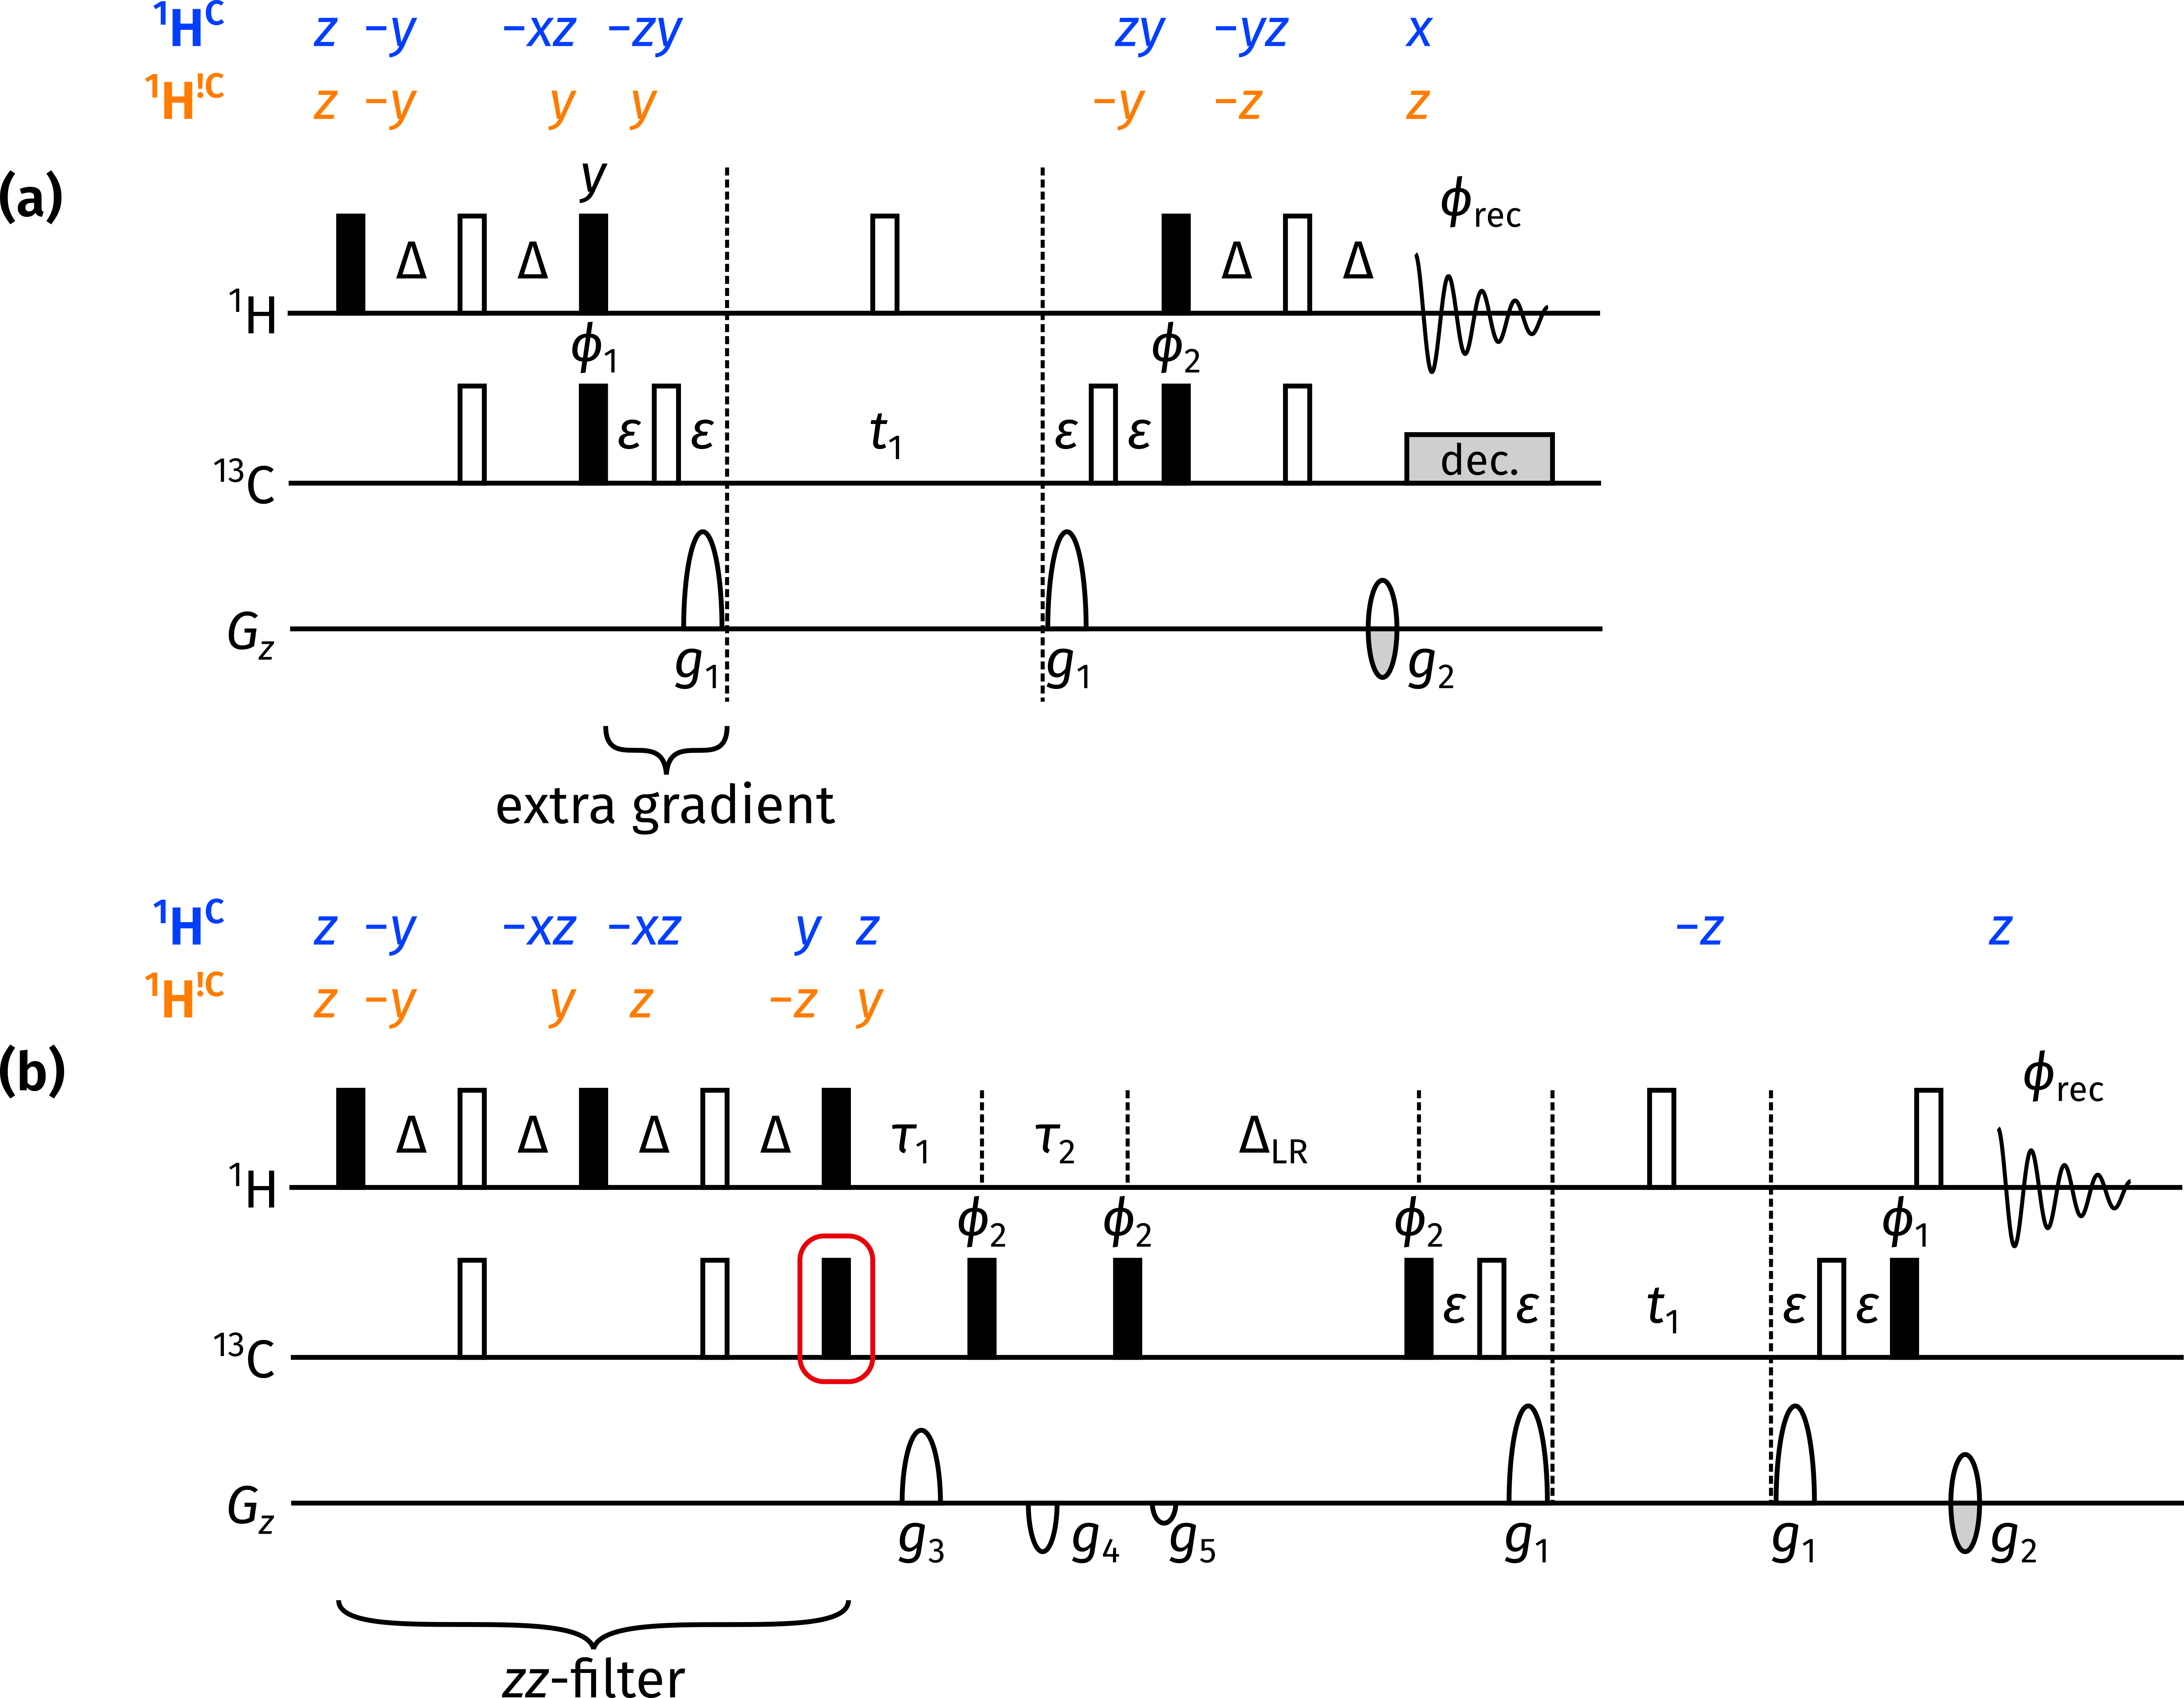
\includegraphics[]{noah/hsqc_hmbc_prodops.png}%
    {\phantomsubcaption\label{fig:noah_sb_po_s}}%
    {\phantomsubcaption\label{fig:noah_sb_po_b}}%
    \caption[NOAH HSQC and HMBC modules with product operator analysis]{
        \textbf{(\subref{fig:noah_sb_po_s})} 
        NOAH HSQC module.
        \textbf{(\subref{fig:noah_sb_po_b})} 
        NOAH HMBC module.
        The \ang{90} pulse highlighted in red is described in \cref{subsec:noah__hmbc}.
        Delays are set as: $\Delta = 1 / (4 \cdot \oneJ{CH})$; $\Delta_\text{LR} = 1 / (2 \cdot \nJ{CH})$; $\tau_1 = 1 / (2 \cdot \oneJ{CH,\text{max}})$; $\tau_2 = 1 / (2 \cdot \oneJ{CH,\text{min}})$ (see also \cref{subsec:poise__hmbc} for the LPJF).
        Phase cycling is performed with $\phi_1 = (x, -x)$, $\phi_2 = (x, x, -x, -x)$, and $\phi_\text{rec} = (x, -x, -x, x)$.
        Gradient amplitudes are $(g_1, g_2, g_3, g_4, g_5) = (80\%, \pm 40.2\%, 15\%, -10\%, -5\%)$.
        Product operator analysis is provided above both modules for both the \magn{C} and \magnnot{C} magnetisation pools; the notation for this is explained in the \textit{Preface}.
    }
    \label{fig:noah_sb_po}
\end{figure}

Sometimes, the modifications required are more extensive, as in the HMBC module.
If this module is followed by a HSQC module (or any other module which draws on \magn{C} magnetisation), the initial \ang{90} excitation pulse must be replaced with a $zz$-filter (\cref{fig:noah_sb_po_b}).
This performs an \textit{isotope-selective rotation} in that \magn{C} magnetisation is stored along the $z$-axis, but \magnnot{C} magnetisation is excited (and subsequently detected).
In general, sequences which are thus modified have lower sensitivities (i.e.\ $A < 1$) than the `original' sequences from which they were derived.
This is partly because of imperfect manipulation of magnetisation by the extra pulse sequence elements, and also increased losses due to relaxation during these extended sequences.

In contrast, modules placed towards the \textit{end} of a supersequence do not need to be modified, as they do not need to preserve any magnetisation.
This includes virtually all homonuclear modules, which are allowed to simply consume any remaining magnetisation.
Although this makes their implementation very straightforward, in general these modules will \textit{also} suffer some losses in sensitivity, because the preceding modules do not perfectly retain all magnetisation.

Thus, in general, it is not possible for any module in a NOAH supersequence to have $A = 1$, unless it is placed first in the supersequence \textit{and} has not undergone any modifications.%
\footnote{Of course, this also depends on exactly \textit{what} standalone experiment the NOAH supersequence is being compared against. Sometimes, in the literature, the NOAH experiment has been compared against its constituent modules acquired in a standalone fashion; in this case, the first module will always have $A = 1$. This tells us how much we gain through the act of concatenating modules, but is less meaningful in the `real world' where one is interested in how useful NOAH is relative to `typical' optimised 2D experiments. I therefore prefer to make comparisons against standard-library sequences.}
Such cases are very rare, and it is thus necessary to accept some decreases in $A$, which are often fairly small (on the order of 10--20\%).
In the sampling-limited regime, sensitivity is not at a premium and this is often perfectly tolerable.
In the sensitivity-limited regime, the full time savings $\rho_t$ cannot be realised, but since $\varepsilon$ is still typically larger than 1, there is still an overall boost in sensitivity per unit time.

\subsection{Case studies}
\label{subsec:noah__case_studies}

Using all that has been described in the previous sections, we now look at a few `typical' supersequences to understand their construction.
A quick note about the nomenclature of NOAH supersequences is warranted here.
Supersequences are labelled by the number of modules $N$, plus a series of single-letter codes corresponding to the identity and ordering of the modules involved (\cref{tbl:noah_modules}).
Occasionally, superscripts or subscripts are used to qualify the modules involved.%
\footnote{With the increasing number of modules, and the variety of modern NMR experiments which could be incorporated into NOAH supersequences, keeping these abbreviations short yet meaningful has been a challenge.}
Thus, a NOAH supersequence containing three modules---say \nitrogen{} HMQC, \carbon{} HSQC, and CLIP-COSY---would be referred to as a \noah{Mn,S,Cc}.
\Cref{tbl:noah_sensitivities} provides values of $\rho_t$ and $A$ for each module of several typical supersequences, which will be rationalised in the text which follows.

\begin{table}[!ht]
    \begin{tabular}{cccccc}
        \toprule
        \multicolumn{2}{c}{\textbf{\proton{}--\nitrogen{} modules}}  &
        \multicolumn{2}{c}{\textbf{\proton{}--\carbon{} modules}}    &
        \multicolumn{2}{c}{\textbf{\proton{}--\proton{} modules}}   \\
        \cmidrule(lr){1-2}
        \cmidrule(lr){3-4}
        \cmidrule(lr){5-6}
        Module & Code        & Module     & Code           & Module     & Code       \\
        \midrule
        HMQC   & \noah*{Mn}  & HSQC       & \noah*{S}      & COSY       & \noah*{C}  \\
        HSQC   & \noah*{Sn}  & seHSQC     & \noah*{Sp}     & CLIP-COSY  & \noah*{Cc} \\
        seHSQC & \noah*{Spn} & HSQC-TOCSY & \noah*{St}     & DQF-COSY   & \noah*{D}  \\
        HMBC   & \noah*{Bn}  & HSQC-COSY  & \noah*{Sc}     & TOCSY      & \noah*{T}  \\
               &             & 2BOB       & \noah*{O}      & NOESY      & \noah*{N}  \\
               &             & HMBC       & \noah*{B}      & ROESY      & \noah*{R}  \\
               &             & ADEQUATE   & \noah*{A}      & PSYCHE     & \noah*{P}  \\
               &             &            & \hspace{1.5cm} & TSE-PSYCHE & \noah*{Pt} \\
               &             &            &                & PSYCHE 2DJ & \noah*{J}  \\
        \bottomrule
    \end{tabular}
    % The hspace is to make the two subcolumns look more balanced.
    \caption[List of single-letter NOAH module codes]{
        A (non-exhaustive) list of single-letter module codes for a selection of NOAH modules.
        Note that, in the literature, the \nitrogen{} HMQC module has been referred to simply by `M', since the HSQC module is preferred for \proton{}--\carbon{} correlations.
        In this thesis, I include the subscript N throughout to avoid any ambiguity.
    }
    \label{tbl:noah_modules}
\end{table}

\begin{table}[!ht]
    % data is in lab book: noah-misc/220224/
    \begin{tabular}{ccccccccc}
        \toprule
        \textbf{Entry} & \textbf{Sequence} & $\symbf{\tau}_{\textbf{NOAH}}$ & $\symbf{\rho}_{\symbfit{t}}$ & \multicolumn{5}{c}{$\symbfit{A}$} \\
        \cmidrule(lr){5-9}
        & & & & HMBC & seHSQC & HSQC & COSY & TOCSY \\
        \midrule
        1 & \noah*{S,C}         & 15 min 0 s  & 1.87 &      &      & 0.97 & 0.90 &      \\
        2 & \noah*{S,C,T}       & 16 min 25 s & 2.60 &      &      & 1.01 & 0.99 & 0.79 \\
        3 & \noah*{B,S}         & 15 min 40 s & 1.82 & 0.93 &      & 0.87 &      &      \\
        4 & \noah*{S,B}         & 15 min 35 s & 1.83 & 0.99 &      & 0.96 &      &      \\
        5 & \noah*{B,S,C,T}     & 17 min 48 s & 3.22 & 0.95 &      & 0.90 & 0.36 & 0.28 \\
        6 & \noah*{B,Spn,S,C,T} & 18 min 57 s & 3.74 & 0.95 & 0.71 & 0.66 & 0.38 & 0.30 \\
        7 & \noah*{Spn,B,S,C,T} & 18 min 56 s & 3.75 & 0.76 & 0.79 & 0.74 & 0.33 & 0.26 \\
        \bottomrule
    \end{tabular}
    \caption[Sensitivity and time-saving analyses of several NOAH supersequences]{
        Sensitivity and time-saving analyses of several typical NOAH supersequences.
        All experiments were acquired with 2 scans per increment, 256 $t_1$ increments, an acquisition time of \qty{67}{\ms}, and a recovery delay of \qty{1.5}{\s}.
        The HMBC module used here includes the extra \carbon{} \ang{90} pulse described later in \cref{subsec:noah__hmbc}: this has no significant impact on the SNR, and is only mentioned as a technicality.
        The \nitrogen{} seHSQC module is that described in \cref{subsec:noah__sehsqc_n}.
        The CT module here was run with States indirect-dimension quadrature detection, and the individual C module (in entry 1) with echo--antiecho.
        The following Bruker library sequences were used as the `conventional' experiments: \texttt{hmbcetgpl2nd}, \texttt{hsqcetf3gpsi2}, \texttt{hsqcetgpsp.2}, \texttt{cosygpqf}, and \texttt{dipsi2gpphzs}.
        \datacode{7Z-220224}
    }
    \label{tbl:noah_sensitivities}
\end{table}

\subsubsection{\noah{S,C}: HSQC + COSY}

We begin with perhaps the simplest example of a NOAH supersequence, one containing the HSQC and COSY modules: this is labelled as a \noah{S,C} experiment (entry 1, \cref{tbl:noah_sensitivities}).
As shown in \cref{fig:noah_sb_po_s}, the HSQC module only samples \magn{C} magnetisation, and leaves \magnnot{C} magnetisation along the $+z$-axis
Although the HSQC experiment has to be modified to preserve this \magnnot{C} magnetisation, its sensitivity is practically unaffected as compared to a `standard' HSQC ($A = 0.97$).
Furthermore, the COSY module retains \textit{most} of its sensitivity ($A = 0.90$).
The small loss here is because the HSQC module does not \textit{perfectly} preserve the \magnnot{C} magnetisation: for example, evolution of J-couplings as well as relaxation occur during the HSQC pulse sequence, which are ignored in the product operator analysis in \cref{fig:noah_sb_po_s}.

The value of the time-saving factor, $\rho_t = 1.87$, is very close to the theoretical limit of $N = 2$.
This reflects the fact that the pulse sequence itself, $\tau_\text{ps}$, is fairly short for both the HSQC and COSY modules; the deviation therefore chiefly arises from the acquisition time, $\tau_\text{acq}$.
In all respects, this is therefore an example of an `ideal' NOAH supersequence, where the combination of two modules provides time savings without compromising on sensitivity.

It is worth pointing out that the order of the modules cannot be reversed: the COSY module cannot be (easily) modified to preserve \magn{C} magnetisation.
In a hypothetical \noah{C,S} supersequence, the later HSQC module would only be able to use magnetisation recovered during the COSY FID, leading to substantial sensitivity drops.

\begin{figure}[!ht]
    \centering
    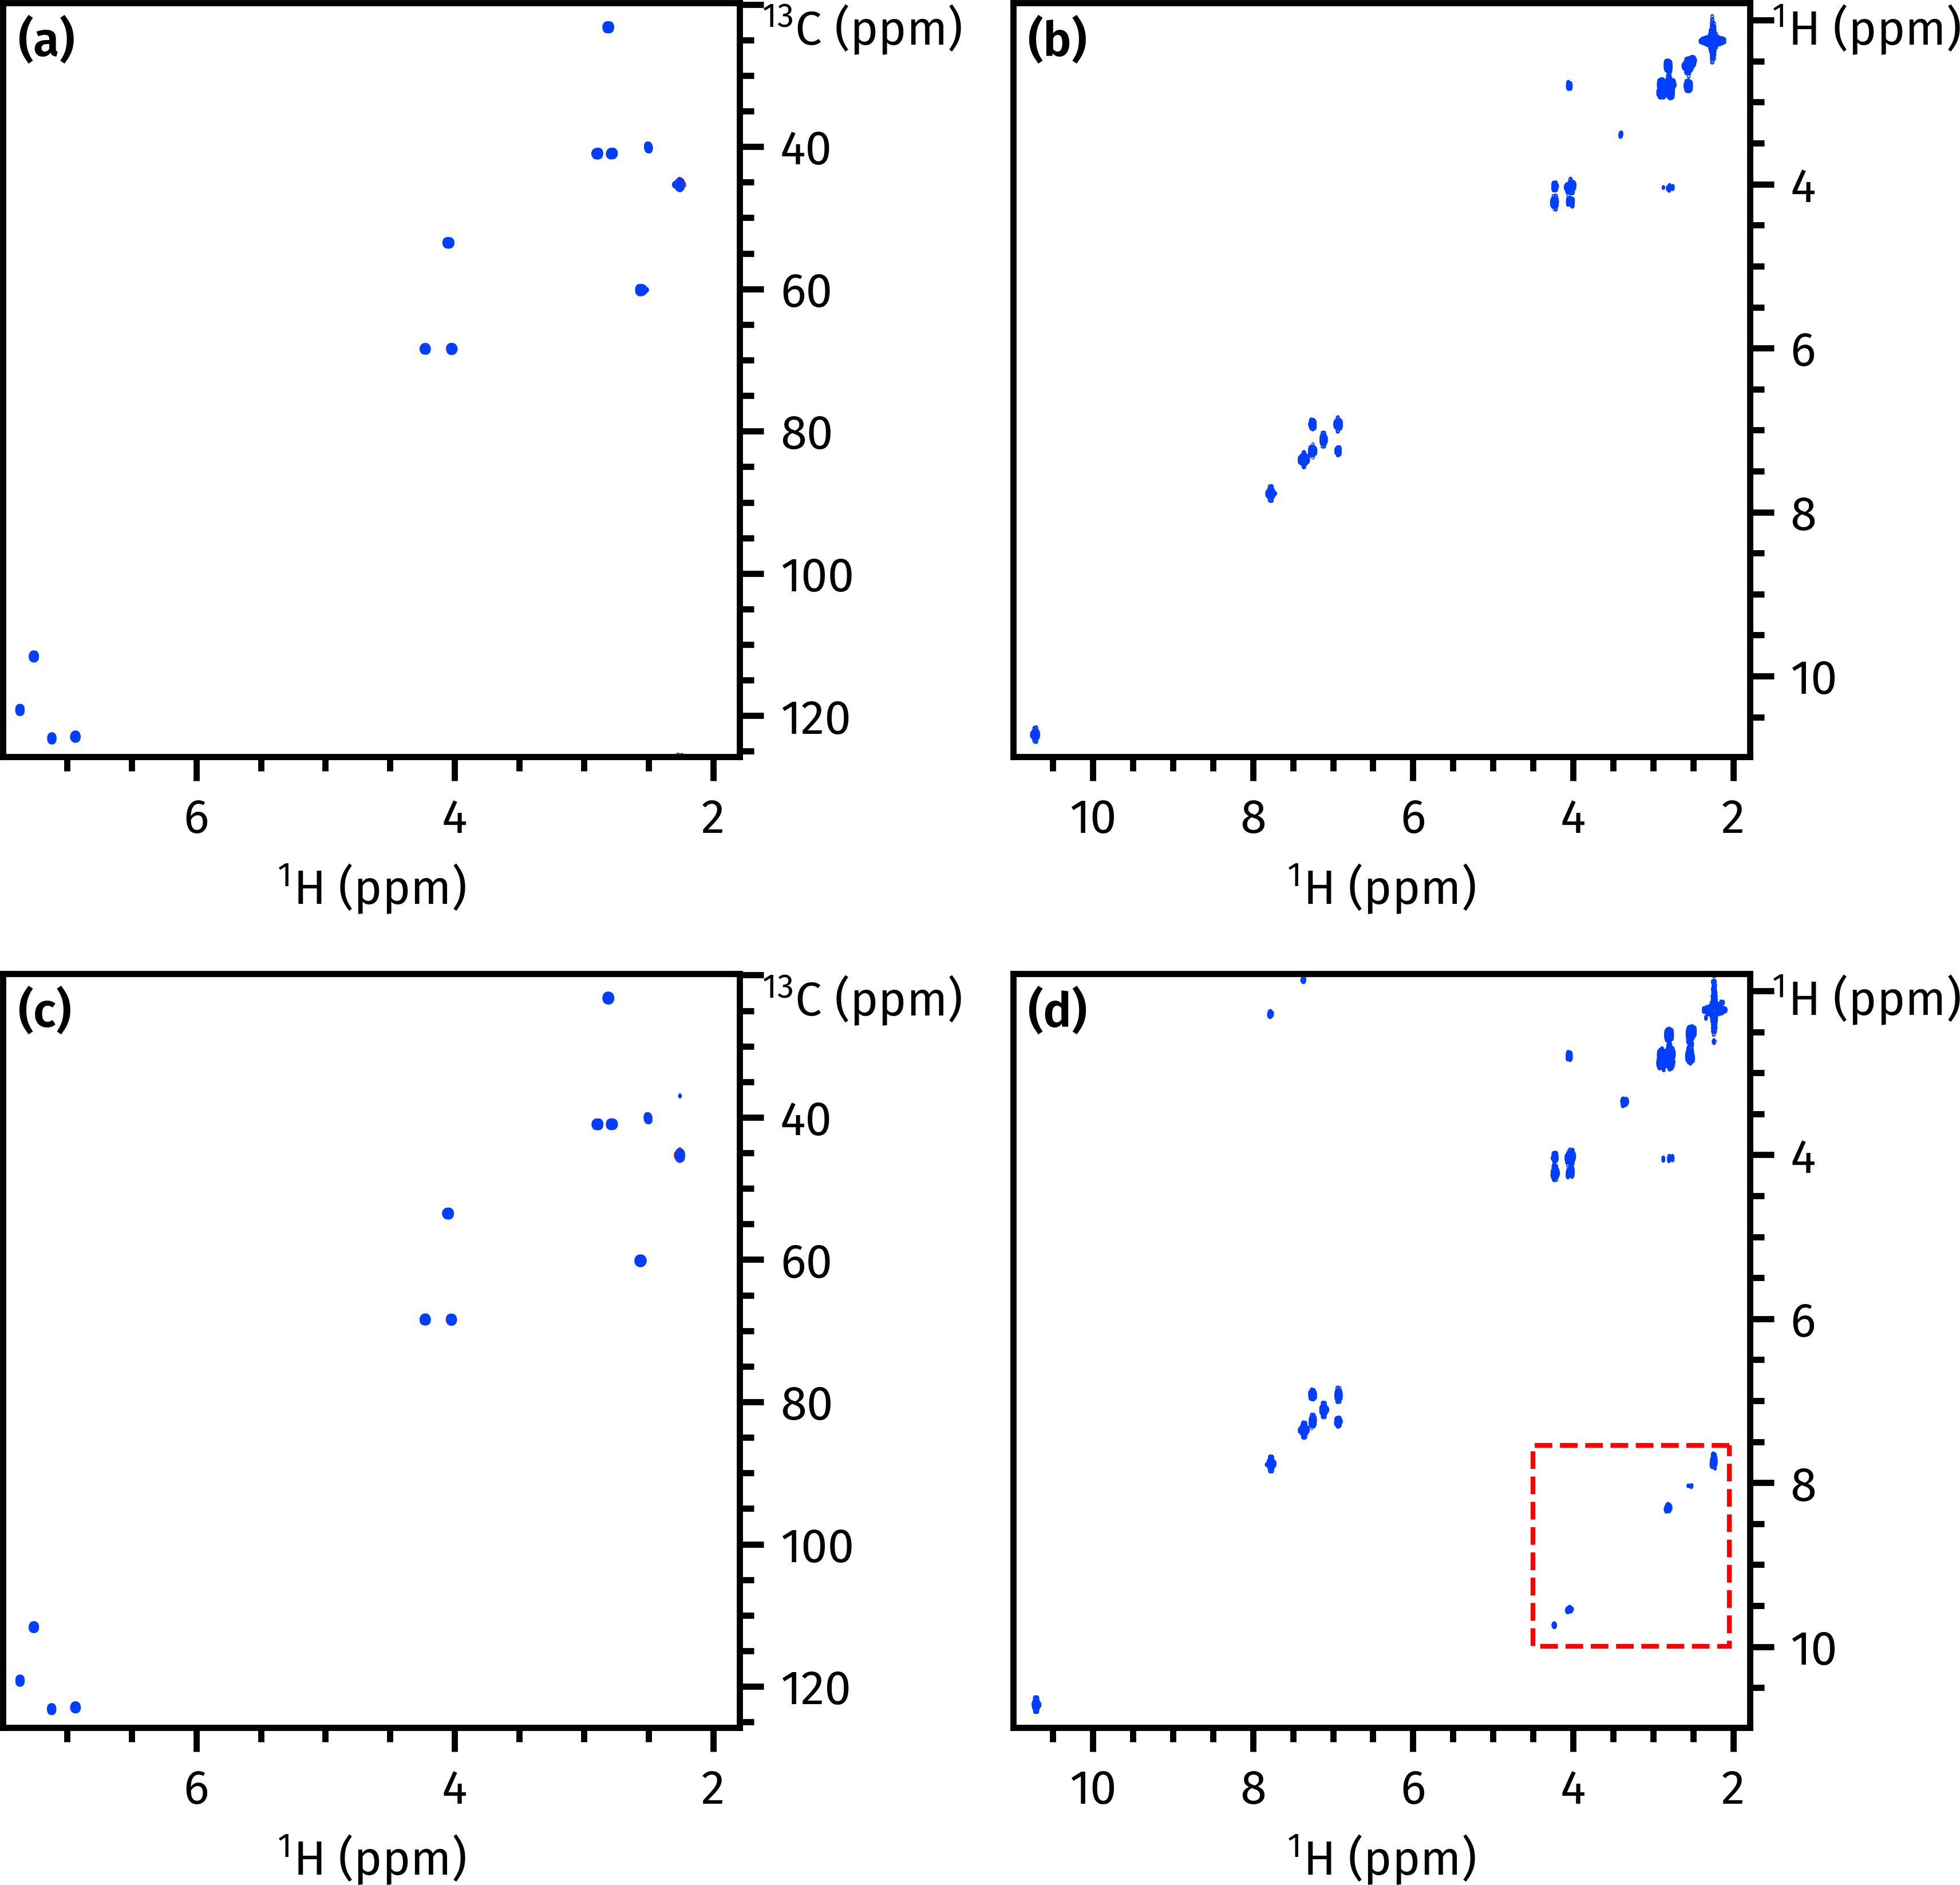
\includegraphics[]{noah/sc_noah_vs_conv.png}%
    {\phantomsubcaption\label{fig:sc_noah_vs_conv_noah_s}}%
    {\phantomsubcaption\label{fig:sc_noah_vs_conv_noah_c}}%
    {\phantomsubcaption\label{fig:sc_noah_vs_conv_conv_s}}%
    {\phantomsubcaption\label{fig:sc_noah_vs_conv_conv_c}}%
    \caption[Comparison of spectra obtained from \noah{S,C} and standalone experiments]{
        \textbf{(\subref*{fig:sc_noah_vs_conv_noah_s})} HSQC from \noah{S,C} supersequence.
        \textbf{(\subref*{fig:sc_noah_vs_conv_noah_c})} COSY from \noah{S,C} supersequence.
        \textbf{(\subref*{fig:sc_noah_vs_conv_conv_s})} Standalone HSQC.
        \textbf{(\subref*{fig:sc_noah_vs_conv_conv_c})} Standalone COSY; off-diagonal artefacts are highlighted in the red box.
        \datacode{7Z-220224}
    }
    \label{fig:sc_noah_vs_conv}
\end{figure}

A final point to consider would be whether the NOAH data has comparable spectral quality in terms of (for example) artefacts.
In this case, the answer is yes: the NOAH HSQC spectrum is virtually identical to the standalone (\cref{fig:sc_noah_vs_conv_noah_s,fig:sc_noah_vs_conv_conv_s}; both spectra have low-level artefacts of different kinds, which do not seriously impede the interpretation and are not shown).
On the other hand, the NOAH COSY spectrum seems to actually \textit{improve} on the standalone COSY, in that it better suppresses off-diagonal artefacts (\cref{fig:sc_noah_vs_conv_noah_c,fig:sc_noah_vs_conv_conv_c}).
These artefacts likely arise in the standalone COSY because of accidental refocusing of magnetisation which has not completely relaxed between $t_1$ increments.\autocite{Vitorge2010JMR}
In contrast, the NOAH COSY module has an extra set of HSQC gradients between every repetition of the COSY, so accidental refocusing is less likely.
(Similar artefacts have been noted before in the DQF-COSY experiment\autocite{Shaw1996JMRSA,Howe2014MRC}, and have also shown to be attenuated in the corresponding NOAH module\autocite{Claridge2019MRC}.)
That said, such improvements are not always guaranteed: there are sometimes artefacts which arise uniquely in NOAH experiments, some of which are discussed in the following sections.


\subsubsection{\noah{S,C,T}: HSQC + COSY + TOCSY}

Evidently, the fact that the HSQC preserves almost all \magnnot{C} magnetisation means that \textit{any} homonuclear module---or a combination thereof---can be placed after it.
In general, since homonuclear modules tend to consume any remaining bulk magnetisation, it is very difficult to create combinations of homonuclear modules which do not lead to significant reductions in sensitivity.
The only real exceptions are COSY/X combinations, where X can be NOESY, ROESY, or TOCSY: instead of concatenating the COSY and X modules, the COSY pulse sequence can instead be nested \textit{within} the X module, as was first demonstrated with X = NOESY\autocite{Haasnoot1984JMR,Gurevich1984JMR}.
Here, we use the COSY/TOCSY combination as an example.\autocite{Nolis2019MRC}
The COSY, TOCSY, and combined COSY/TOCSY modules are shown in \cref{fig:ct_states}.

\begin{figure}[!ht]
    \centering
    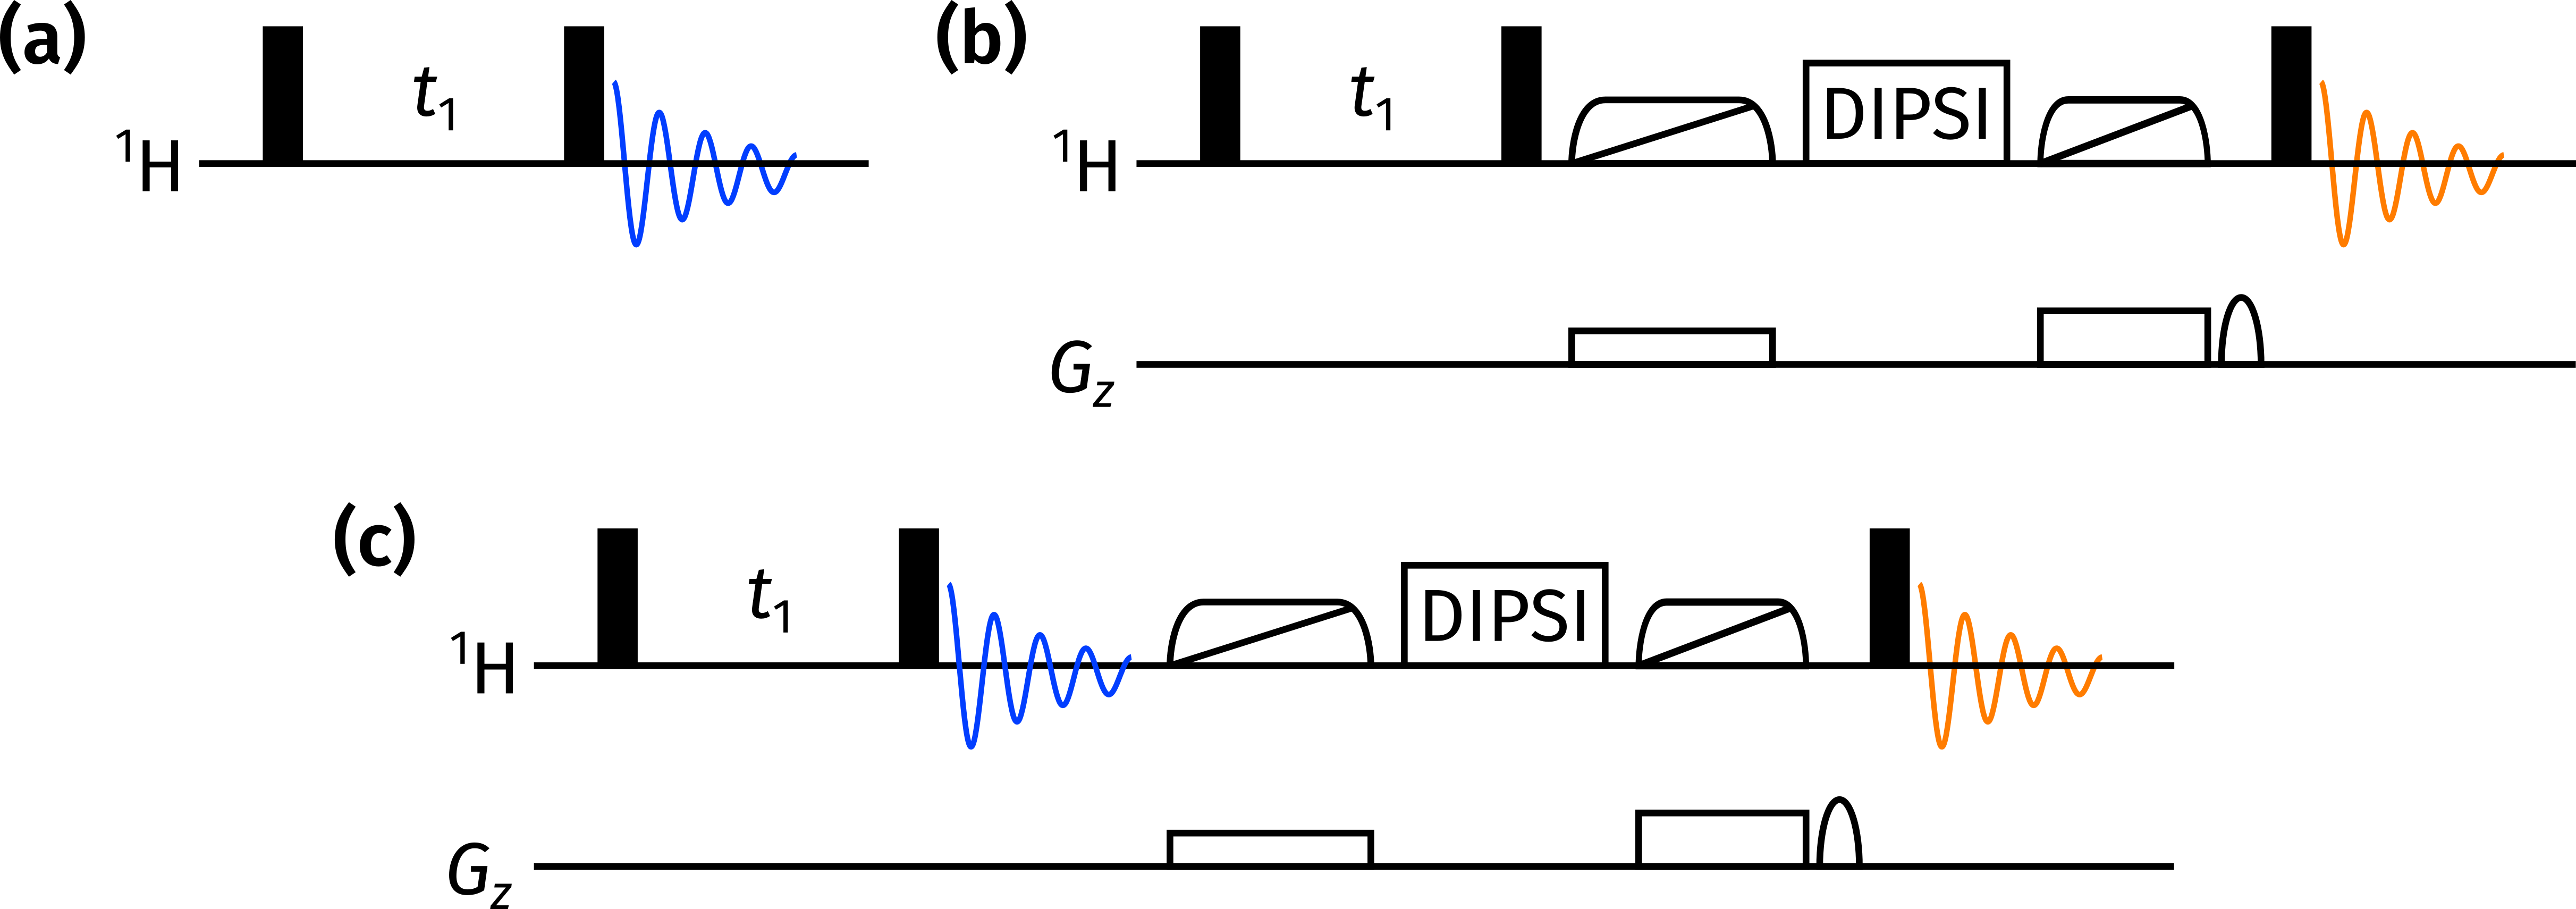
\includegraphics[]{pp/ct_states.png}%
    {\phantomsubcaption\label{fig:ct_states_c}}%
    {\phantomsubcaption\label{fig:ct_states_t}}%
    {\phantomsubcaption\label{fig:ct_states_ct}}%
    \caption[COSY/TOCSY NOAH module]{
        \textbf{(\subref*{fig:ct_states_c})} COSY module.
        \textbf{(\subref*{fig:ct_states_t})} TOCSY module; zero-quantum suppression is employed before and after the isotropic mixing period.
        \textbf{(\subref*{fig:ct_states_ct})} Combined COSY/TOCSY module, where the COSY FID is acquired immediately before the TOCSY mixing.
    }
    \label{fig:ct_states}
\end{figure}

As shown in \cref{tbl:noah_sensitivities} (entry 2), this nesting of the COSY module does not materially affect the TOCSY sensitivity.
A small loss of approximately 20\% is observed, which is partly due to the imperfect magnetisation preservation by the HSQC, and perhaps also due to relaxation during the COSY acquisition period.
As for the time-saving factor, a slightly larger deviation ($\rho_t = 2.60$) is observed from the ideal value of $3$.
This reflects the addition of a TOCSY mixing period, which contributes to $\tau_\text{ps}$.

\subsubsection{\noah{B,S}: HMBC + HSQC}

As mentioned previously, the HMBC module shown in \cref{fig:noah_sb_po_b} is designed to retain \magn{C} magnetisation through the addition of the $zz$-filter.
This can be used in a subsequent HSQC module in a \noah{B,S} supersequence.
Entry 3 of \cref{tbl:noah_sensitivities} shows that the addition of the $zz$-filter to the HMBC causes a relatively small 7\% decrease in sensitivity; on the other hand, the HSQC loses 13\% of its sensitivity because of incomplete magnetisation preservation.

Generally, it has been recommended that less sensitive modules are placed earlier in the supersequence so that they can access a larger proportion of the equilibrium magnetisation.
Since the HMBC is less sensitive of the two modules, this rule of thumb suggests that the BS supersequence would be better than the alternative SB supersequence.
In fact, the opposite is true, as entry 4 of \cref{tbl:noah_sensitivities} shows.
The HSQC module has a boost in sensitivity because it is placed first in the supersequence, and no longer needs to rely on the \magn{C} magnetisation preserved by the HMBC; and the HMBC also benefits because the $zz$-filter modification is no longer needed.%
\footnote{In fact, the final \ang{180} pulse in the HMBC module could also be removed: this is likely to give a further boost in SNR, as discussed in \cref{subsec:noah__hmbc}. However, this was not done here.}
Arguably, the ordering of modules in a supersequence should be considered on a case-by-case basis.

\subsubsection{\noah{B,S,C,T}: HMBC + HSQC + COSY + TOCSY}

We now move on to a longer supersequence containing four modules, with a correspondingly larger $\rho_t$ value of 3.22.
The sensitivity of the HSQC module is practically the same as in the \noah{B,S} supersequence just described: however, the COSY and TOCSY modules expose one weakness of the HMBC module which has so far been overlooked.
In principle, the HMBC module should only excite magnetisation of protons which are long-range coupled to \carbon{} (which we could, for example, denote as \magn{C(LR)}).
This magnetisation pool should be separate from both the directly coupled protons (\magn{C}), as well as protons which are not coupled to any \carbon{} at all (\magnnot{C}).
Unfortunately, this is not the case: it is not actually possible to separate the \magn{C(LR)} and \magnnot{C} magnetisation pools.
The HMBC excites both of these magnetisation sources, dephases the latter using CTP gradients, and detects the signal arising from the former.

What this means, of course, is that the COSY/TOCSY module which rely on \magnnot{C} magnetisation will have substantially lower sensitivities.
The signal detected in these two modules derives only from whatever has recovered during the previous two acquisition periods, as shown in entry 5 of \cref{tbl:noah_sensitivities}: $A$ for COSY and TOCSY is 0.36 and 0.28 respectively.
That said, this is in fact not likely to be an issue \textit{even} for sensitivity-limited samples.
Because the intrinsic sensitivity of the HMBC is orders of magnitude lower than the COSY and TOCSY, even with these large losses in sensitivity, the COSY and TOCSY spectra still have greater intensities than the HMBC.
Thus, as long as the entire supersequence is acquired with enough scans to make the HMBC SNR sufficient, the SNR in the COSY and TOCSY will \textit{also} be acceptable.
This is illustrated in \cref{fig:bsct}.

A rather more insidious problem is that different signals relax at different rates: thus, the COSY and TOCSY spectra (or indeed, any homonuclear module) will have uneven intensities and are frequently asymmetric.
This can be seen in the COSY spectrum, where a pair of asymmetric crosspeaks are highlighted.
Adding a period of isotropic mixing before the COSY module\autocite{Kupce2018CC} can help to ameliorate this to some extent (this was not performed when acquiring the data in \cref{fig:bsct}).

\begin{figure}[!ht]
    \centering
    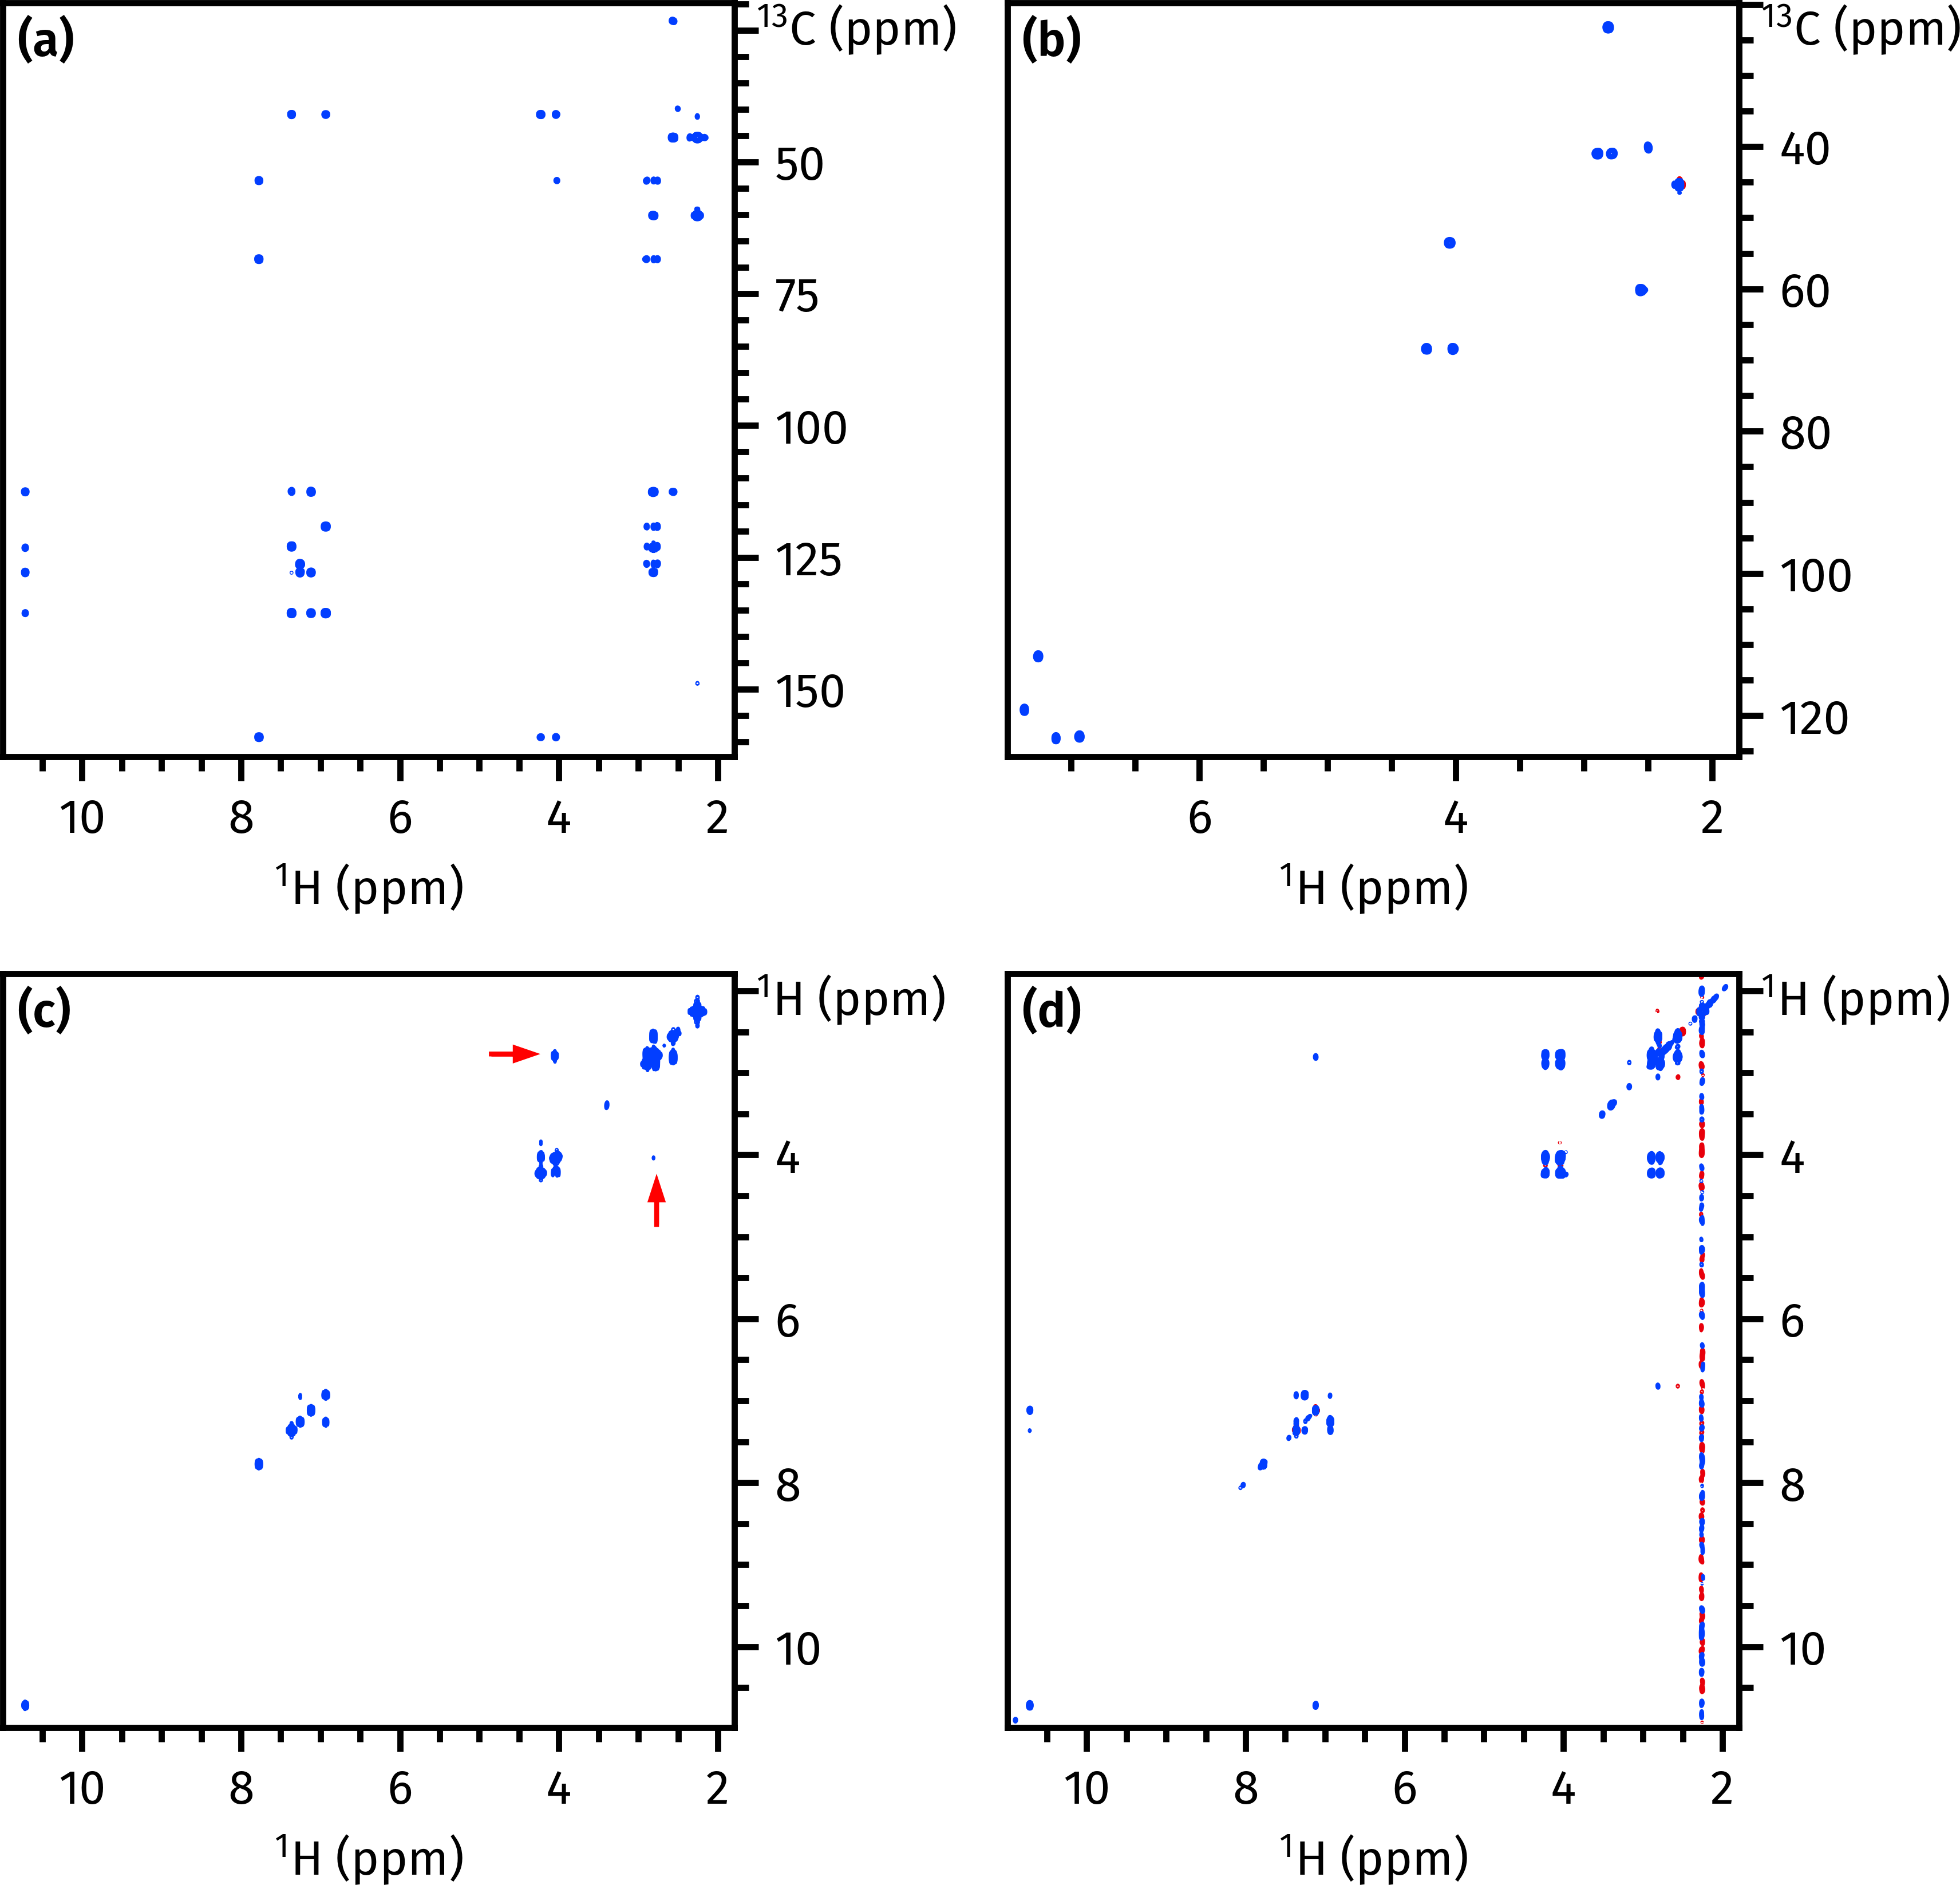
\includegraphics[]{noah/bsct.png}%
    {\phantomsubcaption\label{fig:bsct_b}}%
    {\phantomsubcaption\label{fig:bsct_s}}%
    {\phantomsubcaption\label{fig:bsct_c}}%
    {\phantomsubcaption\label{fig:bsct_t}}%
    \caption[Spectra obtained from a \noah{B,S,C,T} supersequence.]{
        Spectra obtained from a \noah{B,S,C,T} supersequence. 
        \textbf{(\subref*{fig:bsct_b})} HMBC.
        \textbf{(\subref*{fig:bsct_s})} HSQC.
        \textbf{(\subref*{fig:bsct_c})} COSY; a pair of asymmetric crosspeaks are highlighted with red arrows.
        \textbf{(\subref*{fig:bsct_t})} TOCSY (\qty{60}{\ms} DIPSI-2 mixing).
        Despite the COSY and TOCSY having only around 30\% of their sensitivity compared to standalone experiments, the intensity of the spectra obtained is still perfectly acceptable (the contour levels chosen are 1--2 orders of magnitude larger than for the HMBC).
        \datacode{7Z-220224}
    }
    \label{fig:bsct}
\end{figure}


\subsubsection{\noah{B,Spn,S,C,T}: HMBC + \nitrogen{} seHSQC + HSQC + COSY + TOCSY}

As the final example, we add a further magnetisation pool to the mix, namely protons directly coupled to \nitrogen{} (i.e.\ \magn{N}).
As of the time of writing, the implementation of multiple-FID experiments on Bruker spectrometers limits $N$ to a maximum of 5, so a supersequence such as the present \noah{B,Spn,S,C,T} is the current limit.
(However, there is no \textit{scientific} argument forbidding $N > 5$, and it is likely that in future versions of TopSpin this restriction will be lifted.)

The values of $A$ for each module are given in entry 6 of \cref{tbl:noah_sensitivities}.
If the HMBC module is placed at the beginning of the supersequence, then in order to preserve \textit{both} \magn{N} and \magn{C} magnetisation, the $zz$-filter must be extended to include \nitrogen{} pulses\autocite{Kupce2019JMR}.
As before, the \nitrogen{} seHSQC and \carbon{} HSQC modules both suffer drops in sensitivity.
For the \nitrogen{} seHSQC, this is partly because of imperfect preservation of \magn{N} magnetisation by the HMBC, but also stems from the addition of the $zz$ isotope-selective pulse (ZIP) element to the seHSQC pulse sequence; this is described further in \cref{subsec:noah__sehsqc_n}.
On the other hand, for the \carbon{} HSQC, the sensitivity loss stems purely from imperfect retention of \magn{C} magnetisation.
Finally, because the HMBC dephases \magn{!X} magnetisation, the COSY and TOCSY at the end have lower sensitivities: however, as discussed above, this is not an issue in practice.

It is also possible to move the \nitrogen{} seHSQC module to the front: this gives it a slightly greater sensitivity, at the cost of the HMBC (entry 7, \cref{tbl:noah_sensitivities}).
In general, these two modules tend to have comparable sensitivity, and which of these two arrangements is better depends on which module the sensitivity needs to be optimised for.

Lastly, the value of $\rho_t$ given here of 3.74 represents an effective upper limit on the time-saving factor.
Although $\rho_t$ increases with $N$, the extent to which it deviates from the ideal value of $N$ also increases: it is very difficult to obtain $\rho_t > 4$, even with five modules in the supersequence.
Of course, it is possible to increase $\rho_t$ further by lengthening the recovery delay $d_1$ used for the experiments: for example, if $d_1$ is increased to \qty{2}{\s} from its present value of \qty{1.5}{\s}, $\rho_t$ increases to 3.94.
Obviously, this can only be pushed so far before it becomes meaningless.

